% $Id: INF_Poster.tex 7714 2011-08-31 17:34:46Z tkren $
%
% TU Wien - Faculty of Informatics
% poster template
%
% This template is using the beamer document class and beamerposter package, see
% <http://www.ctan.org/tex-archive/macros/latex/contrib/beamer/>
% <http://www.ctan.org/tex-archive/macros/latex/contrib/beamerposter/>
% <http://www-i6.informatik.rwth-aachen.de/~dreuw/latexbeamerposter.php>
%
% For questions and comments send an email to
% Thomas Krennwallner <tkren@kr.tuwien.ac.at>
%

\documentclass[final,hyperref={pdfpagelabels=true}]{beamer}

\makeatletter
  \def\beamer@calltheme#1#2#3{%
    \def\beamer@themelist{#2}
    \@for\beamer@themename:=\beamer@themelist\do
    {\usepackage[{#1}]{\beamer@themelocation/#3\beamer@themename}}}

  \def\usefolder#1{
    \def\beamer@themelocation{#1}
  }
  \def\beamer@themelocation{}

\usefolder{style}

\usepackage{style/TUINFPST}
\usepackage{ragged2e}    %% provides \justifyin
\usepackage{sidecap}     %% for images with side captions
\usepackage{wrapfig}

\title[Software Engineering \& Internet Computing]{Concurrent Programming with\\[.2\baselineskip]Actors and Microservices}
% if you have a long title looking squeezed on the poster, just force
% some distance:
% \title[Computational Intelligence]{%
%   Integration of Conjunctive Queries over \\[0.2\baselineskip]%
%   Description Logics into HEX-Programs %\\[0.2\baselineskip]%
% }
\author[max@irro.at]{Maximilian Irro}
\institute[]{%
  Technische Universit{\"a}t Wien\\[0.25\baselineskip]
  Institut f{\"u}r Information Systems Engineering\\[0.25\baselineskip]
  Arbeitsbereich: Compilers and Languages\\[0.25\baselineskip]
  Betreuer: Ao.Univ.Prof. Dipl.-Ing. Dr. Franz Puntigam
}
\titlegraphic{
\includegraphics[height=52mm]{complang-logo-neu}}
\date[\today]{\today}
\subject{epilog}
\keywords{concurrent programming, actor model, microservices}

%%%%%%%%%%%%%%%%%%%%%%%%%%%%%%%%%%%%%%%%%%%%%%%%%%%%%%%%%%%%%%%%%%%%%%%%%%%%%%%%%%%%%%
% Display a grid to help align images 
%\beamertemplategridbackground[1cm]

% for crop marks, uncomment the following line
%\usepackage[cross,width=88truecm,height=123truecm,center]{crop}

%%%%%%%%%%%%%%%%%%%%%%%%%%%%%%%%%%%%%%%%%%%%%%%%%%%%%%%%%%%%%%%%%%%%%%%%%%%%%%%%%%%%%%

\begin{document}

  % We have a single poster frame.
  \begin{frame}

    \newcommand{\lmodern}{\fontfamily{lmr}\selectfont}
    
    \renewcommand\rmdefault{lmr}
    \renewcommand\sfdefault{lmss}
    \renewcommand\ttdefault{lmtt}

    %\renewcommand\rmdefault{lmr}
    %\renewcommand\sfdefault{lmss}
    %\renewcommand\ttdefault{lmtt}

    %\rmfamily % roman font family

    \begin{columns}[t]
      % ---------------------------------------------------------%
      % Set up a column
      \begin{column}{.45\textwidth}
        \textsf{\textbf{INTRODUCTION}} \\
        \vspace*{\baselineskip}
        {\lmodern\justifying
          Concurrent programming manages multiple concerns of an application or system simultaneously. We investigate two different models for introducing concurrent computational units into software architectures. The \textbf{actor model} defines theoretically well-known constructs supporting concurrent, parallel and distributed execution in a transparent way. The \textbf{microservice paradigm} facilitates many principles of the old Unix philosophy by composing complex functionality through small, independent, highly cohesive and loosely coupled executables
        }
      \end{column}
      % ---------------------------------------------------------%
      % end the column

      % ---------------------------------------------------------%
      % Set up a column 
      \begin{column}{.45\textwidth}
        \textsf{\textbf{PROBLEM STATEMENT}} \\
        \vspace*{\baselineskip}
        {\lmodern
          There is yet a gap in the literature that emphasizes the connections between actors and microservices. This work fills this gap with a focus on the concurrent programming aspects. We investigate why actors and microservices qualify for programming concurrency, how the models facilitate concurrent execution, what the expressive capabilities of actors and microservices are, and finally we compare the performance of an actor-based and microservice-based implementation of a non-trivial concurrent system scenario.

        }
      \end{column}
      % ---------------------------------------------------------%
      % end the column
    \end{columns}

    \vspace*{2\baselineskip}

    \begin{columns}[t]
    % ---------------------------------------------------------%
    % Set up a column
    \begin{column}{.45\textwidth}
      \textsf{\textbf{ACTOR MODEL}} \\
      \vspace*{\baselineskip}
      {\lmodern
        Actors encapsulate state exclusively and communicate via asynchronous message passing. All actors live inside a runtime system that concurrently executes them. Actors are passive computational units, since they only react to messages. Exclusive state ownership and isolated message processing results in single-threaded semantics internally. Actors are therefore free of synchronization requirements.
      }
    \end{column}
    % ---------------------------------------------------------%
    % end the column

    % ---------------------------------------------------------%
    % Set up a column 
    \begin{column}{.45\textwidth}
      \textsf{\textbf{MICROSERVICE PARADIGM}} \\
      \vspace*{\baselineskip}
      {\lmodern
        Every microservices is a dedicated operating system process. They communicate via a light-weight, technology-neutral message passing channels. Microservices are executed by an operating system scheduler, which facilitates concurrency and parallelism. Network communication channels additionally result in distribution. Microservices are active units and show behavior on their own accord.
      }
    \end{column}
    % ---------------------------------------------------------%
    % end the column
  \end{columns}

  \vspace*{2\baselineskip}
  
  \begin{columns}[t]
    % ---------------------------------------------------------%
    % Set up a column
    \begin{column}{.45\textwidth}
      \textsf{\textbf{EXPRESSIVENESS \& CAPABILITIES}} \\
      \vspace*{\baselineskip}
      {\lmodern

        Our evaluation shows that both models have the same expressive capabilities regarding concurrent programming concerns. They merely apply different implementation strategies, which come with different trade-offs.
        
        \textbf{\textsf{Encapsulation}}:

        Actors conceptually encapsulate state exclusively. Shared-memory environments practically threaten the isolation. Programmers must ensure that no mutable state is accessible among actors through reference sharing.

        Microservices also encapsulate their state. The paradigm forbids shared memory among services. State is isolated through the strict memory boundaries of system processes that are enforced by the operating system.

        \textbf{\textsf{Communication}}:

        Actors have an asynchronous messaging primitive. Runtimes can provide additional comnunication abstractions. These abstractions have to build on top of the asynchronous primitive. All communication in actor systems is therefore at most semi-synchronous.

        Microservices facilitate technology-neutral communication channels in every interaction style they choose. A channel is valid as long as there is no shared memory, but message passing semantics instead.

        \textbf{\textsf{Concurrent Execution}}:

        Actors and microservices encapsulate their state exclusively and all their communication solely facilitates message passing semantics. These properties make the task units highly cohesive and provide a temporal and spacial decoupling. The resulting independence is the foundation that enables an actor runtime or respectively an operating system to execute the task units in a concurrent fashion implicitly.

        \textbf{\textsf{Scalability}}:
        
      }
    \end{column}
    % ---------------------------------------------------------%
    % end the column

    % ---------------------------------------------------------%
    % Set up a column 
    \begin{column}{.45\textwidth}
      \textsf{\textbf{EFFICIENCY \& BENCHMARK}} \\
      \vspace*{\baselineskip}
      {\lmodern
        We evaluated the efficiency of the programming models with respect to a non-trivial scenario of a concurrent system. Our scenario is a domain-specific search engine, since the architecture provides many opportunities to facilitate concurrent processing. The benchmark results below are for an actor-based and a microservices-based system implementation of this scenario. We used Akka as the actor system and built the microservices on the Spring framework.
      }

      
      \begin{columns}[t]
        \begin{column}{.4\textwidth}
          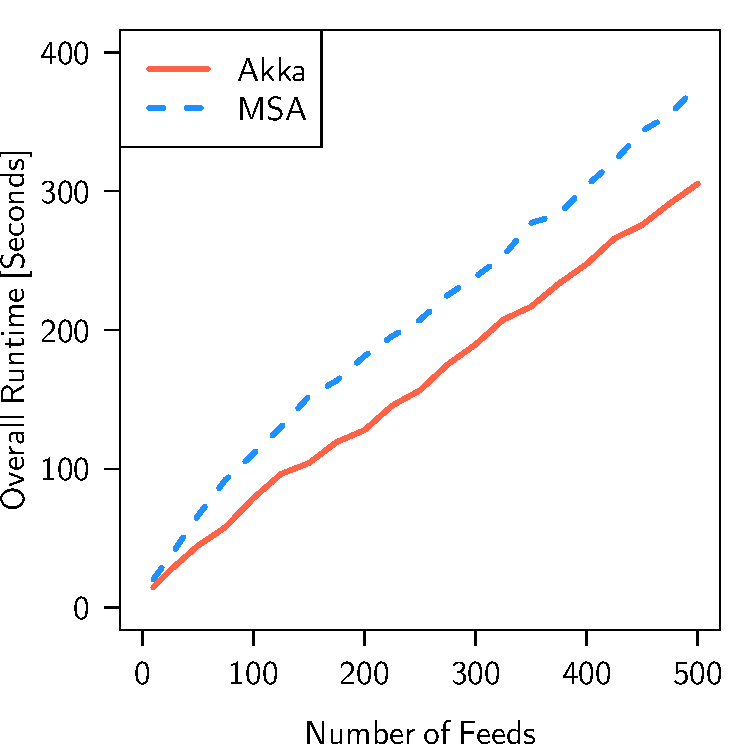
\includegraphics[width=1\textwidth]{graphics/eval-index-overall.pdf}
        \end{column}
        \begin{column}{.05\textwidth}
          % Intentionally left blank
        \end{column}
        \begin{column}{.55\textwidth}
          {\lmodern
            The indexing phase facilitate asynchronous communication. The microservice use RabbitMQ as their channel. The results show that the execution modality of actors is more efficient. Microservices have a higher runtime overhead, since they are separate system processes. 
          }
        \end{column}
      \end{columns}

      \begin{columns}[t]
        \begin{column}{.4\textwidth}
          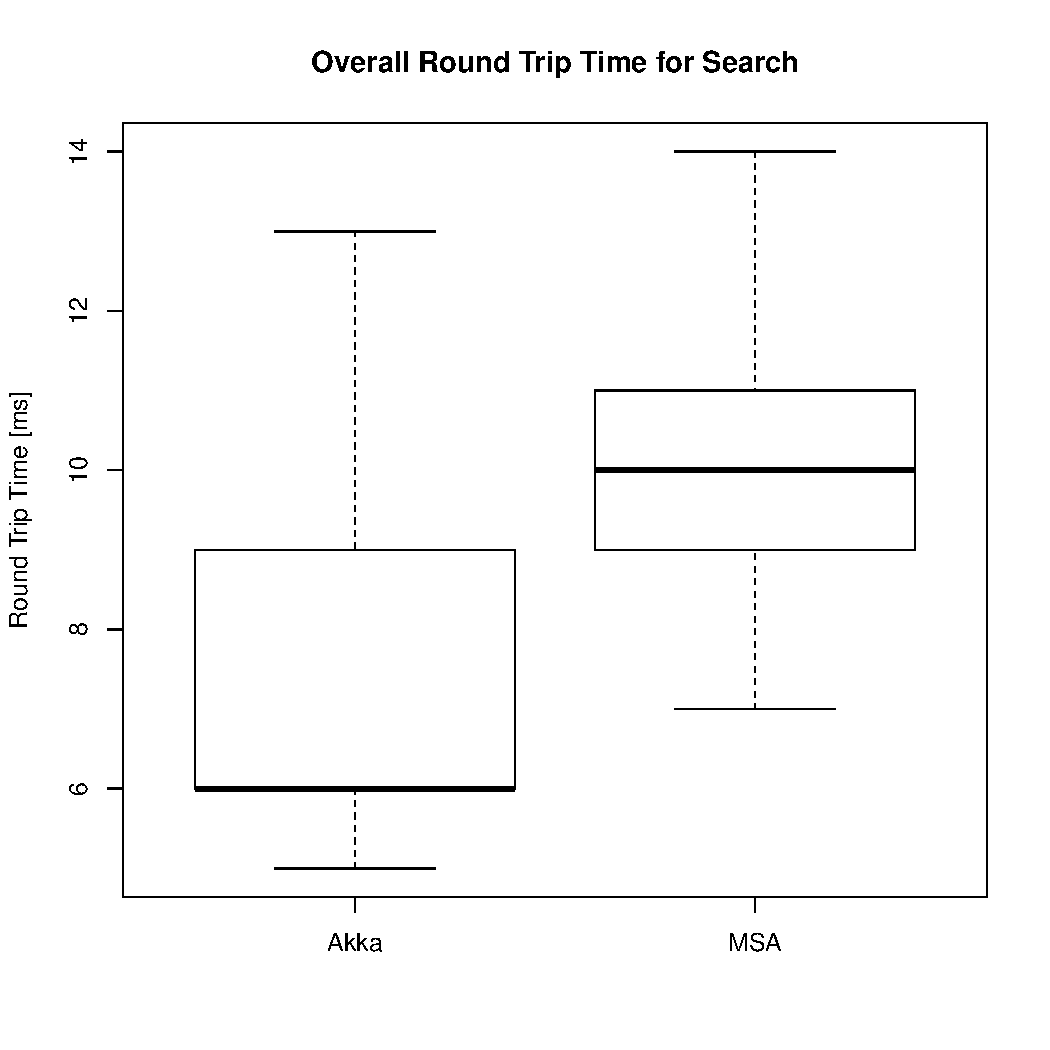
\includegraphics[width=1\textwidth]{graphics/eval-search-rtt-overall.pdf}
        \end{column}
        \begin{column}{.05\textwidth}
          % Intentionally left blank
        \end{column}
        \begin{column}{.55\textwidth}
          {\lmodern

            The retrieval phase requires request/response communication. Actors have to model synchronous interaction with in a request/asynchronous response style. Microservices simply use REST-based communication. The semi-synchronous strategy of actors is clearly more efficient than strictly synchronous communication.  
          }
        \end{column}
      \end{columns}


    \end{column}
    % ---------------------------------------------------------%
    % end the column
  \end{columns}

\end{frame}

\end{document}

%%% Local Variables:
%%% TeX-PDF-mode: t
%%% TeX-debug-bad-boxes: t
%%% TeX-master: t
%%% TeX-parse-self: t
%%% TeX-auto-save: t
%%% reftex-plug-into-AUCTeX: t
%%% End:
